\begin{figure}[h]
	\centering
	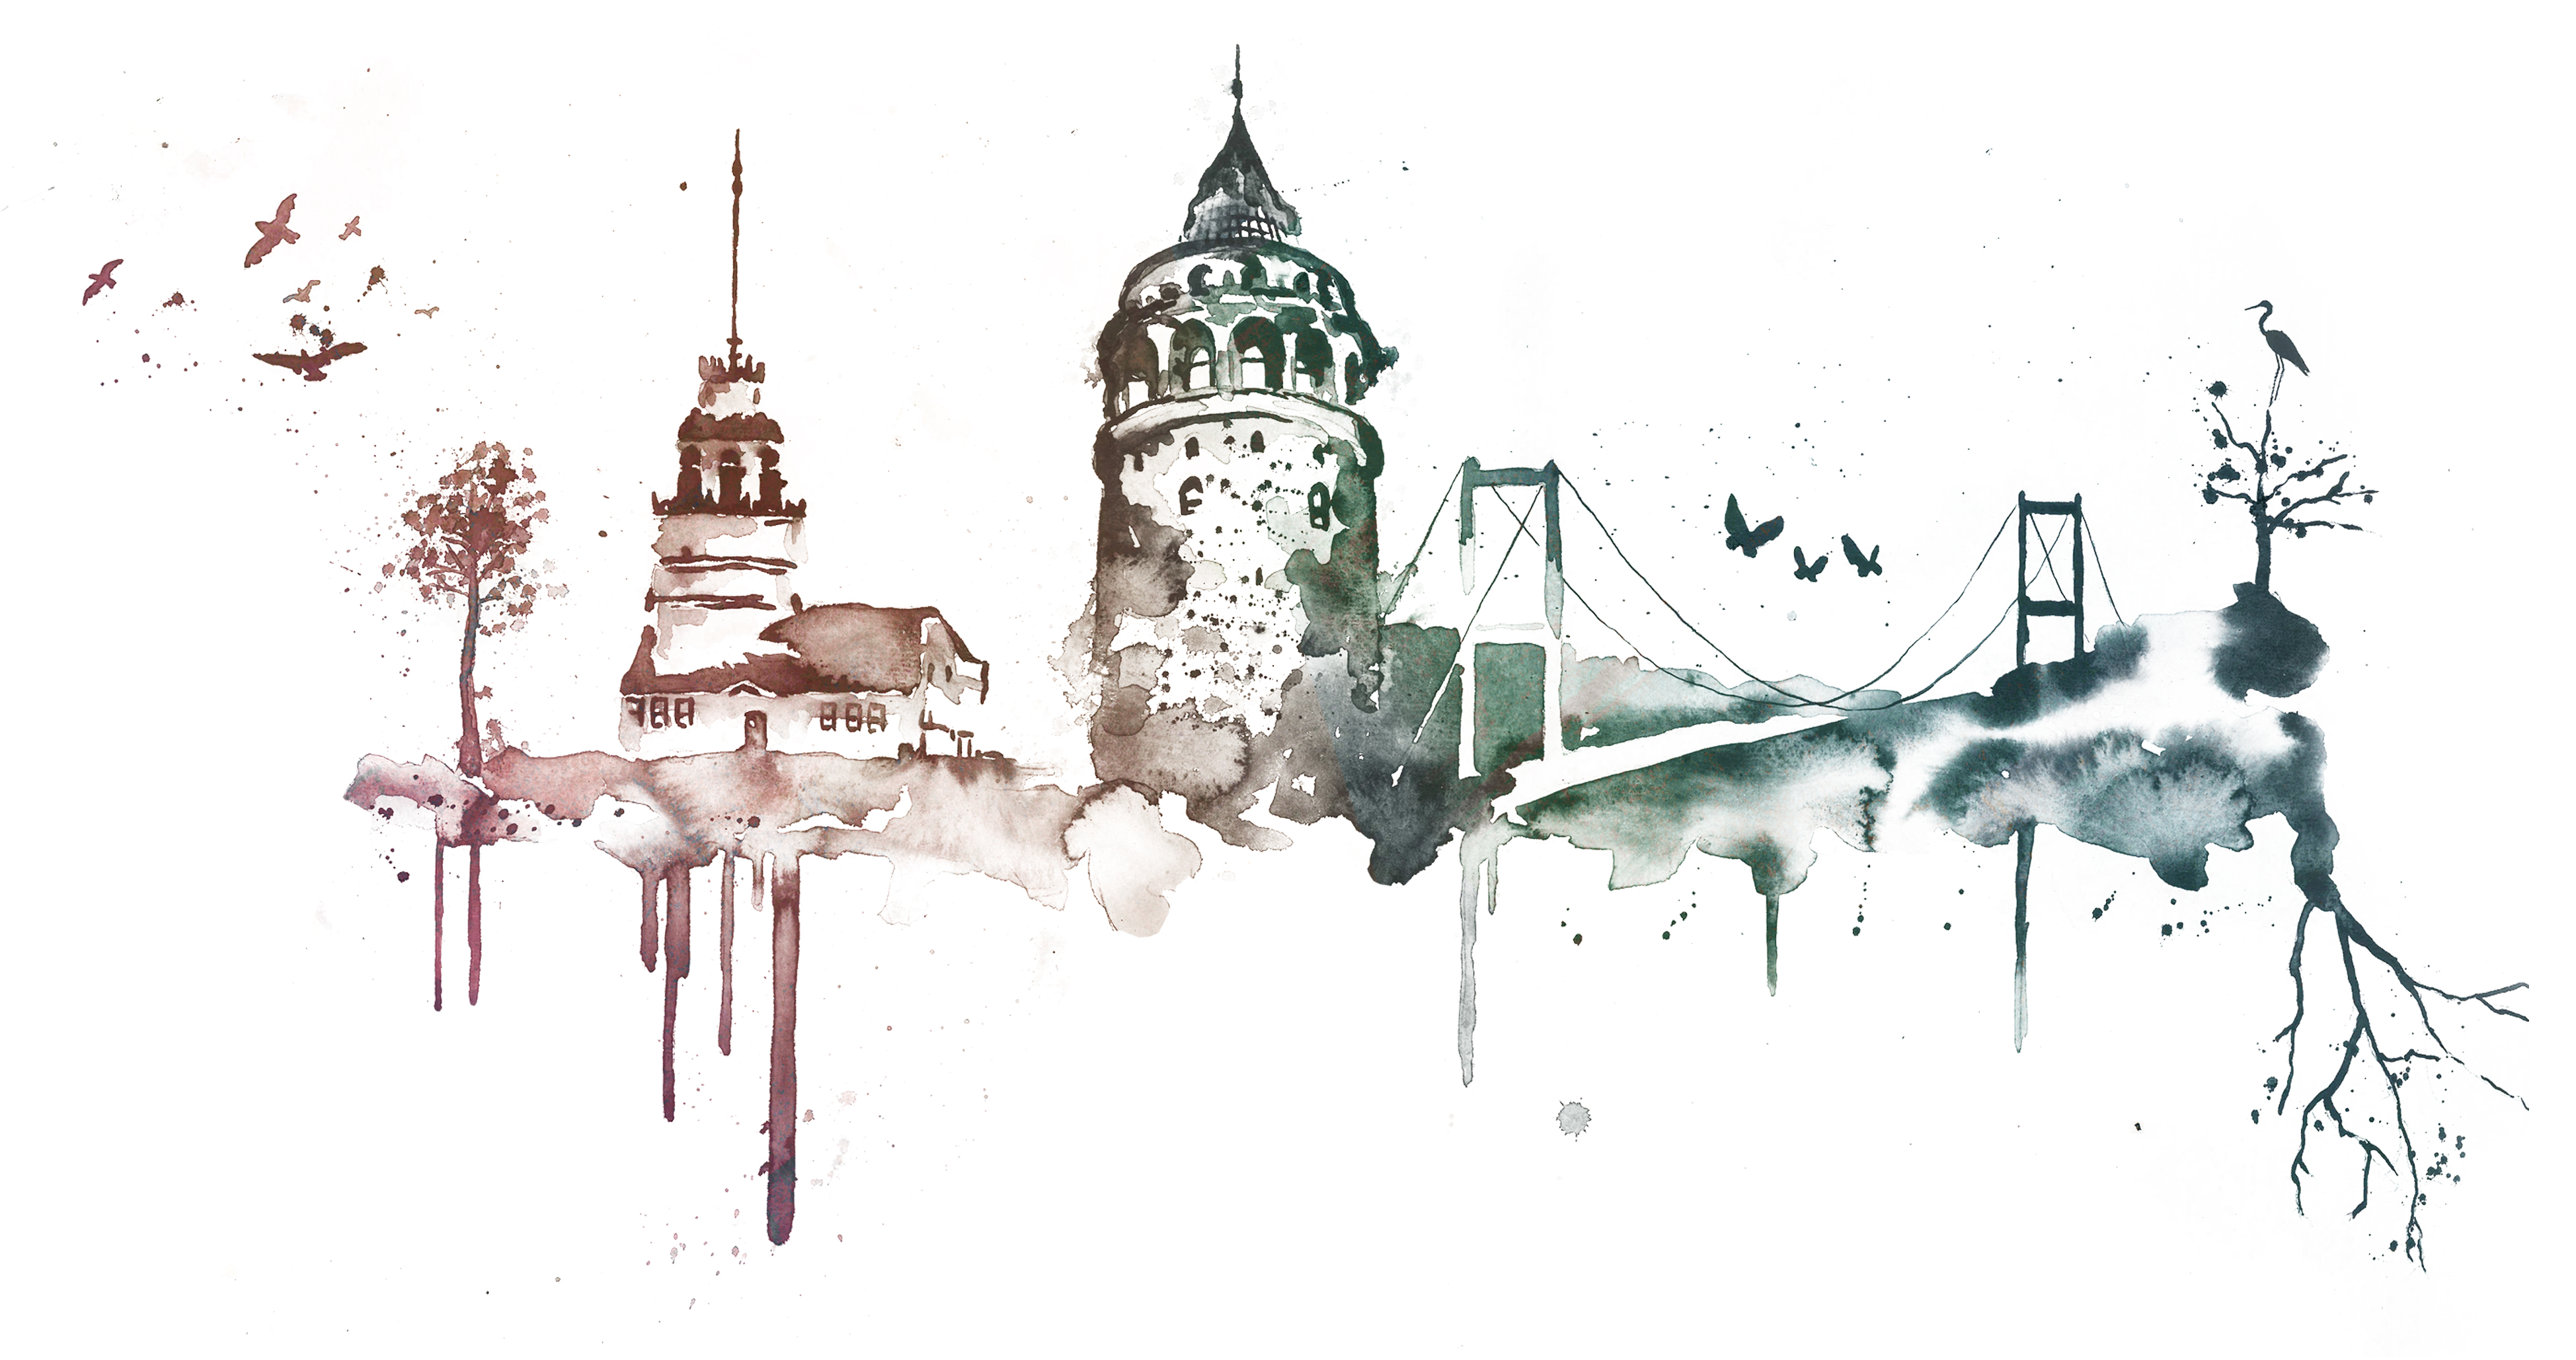
\includegraphics[width=16cm]{./pic/t2-1.png}
\end{figure}

一些元素的名字源于由世界各地的地名。这一点上,瑞典村庄Ytterby创造了一项纪录,四种元素:镱(ytterbium,Yb)、钇(yttrium,Y)、铒(erbium,Er)和铽(terbium,Tb)得名于此。然而,并不仅仅是元素会以地名命名。有趣的是,一系列天然产物\textbf{istanbulin A--E}的名字源于城市伊斯坦布尔。这一系列的前两个成员即istanbulin A和B首次于1971年由教授Ayhan Ulubelen博士及其合作者从植物\emph{Smyrnium olusatrum}(译注:又名亚历山大草)中分离得到。剩下的3个成员即istanbulin C--E由Ulubelen及其合作者在1979年至1982年间报道。

\begin{figure}[h]
	\centering
	\includegraphics[width=12cm]{./pic/t2-2.pdf}
\end{figure}

Istanbulin是倍半萜天然产物这一更大家庭中的一员。Vernolepin \textbf{1}和vernomenin \textbf{2}是两种重要的倍半萜天然产物,它们具有类似的6-6-5并环体系。1976年,Danishefsky及其合作者报道了这两个化合物的全合成。在这一漂亮的全合成路线中,Danishefsky将所谓Danishefsky二烯用于Diels--Alder (DA)反应中。

\begin{figure}[h]
	\centering
	\includegraphics[width=9cm]{./pic/t2-3.pdf}
\end{figure}

请注意本题中所有的手性化合物的结构式都表示外消旋体。
\newpage

上下文中提到的Danishefsky二烯 \textbf{3}和Rawal--Kozmin二烯 \textbf{4}是两个富电子二烯,都已广泛用于有机合成中。它们的结构如下所示:

\begin{figure}[h]
	\centering
	\includegraphics[width=9cm]{./pic/t2-4.pdf}
\end{figure}

TMS: 三甲基硅基;TBS: 叔丁二甲基硅基

\noindent\textbf{2.1.}画出\textbf{3}和\textbf{4}主要的共振式。指出每个二烯中电子密度最高的碳原子。

\noindent\textbf{2.2.}化合物\textbf{3}和\textbf{4}广泛用作Diels--Alder反应的双烯体。画出\textbf{3}和\textbf{4}能够发生DA反应时的构象。推测在与顺丁烯二酸酐\textbf{5}发生DA反应时,哪个二烯的活性更高?

\begin{figure}[h]
	\centering
	\includegraphics[width=4cm]{./pic/t2-5.pdf}
\end{figure}

加热Danishefsky二烯 \textbf{3}与化合物\textbf{6}的混合物,随后用酸(TsOH,对甲苯磺酸)处理,得到主要产物化合物\textbf{A}。

\begin{figure}[h!]
	\centering
	\includegraphics[width=11cm]{./pic/t2-6.pdf}
\end{figure}

\noindent\textbf{2.3.}画出\textbf{3}和\textbf{6}发生Diels--Alder反应所有可能的产物,它们的化学式都为C\textsubscript{12}H\textsubscript{14}O\textsubscript{3}。每一组对映异构体画出其中一种即可。

\noindent\textbf{2.4.} 确定主产物\textbf{A}的结构。

\noindent\textbf{2.5.} Diels--Alder加合物\textbf{A}依次经历如下的4步反应转化为化合物\textbf{7}。化合物\textbf{B}具有酸性。画出\textbf{B}-\textbf{D}的结构。

\begin{figure}[h]
	\centering
	\includegraphics[width=14cm]{./pic/t2-7.pdf}
\end{figure}

\noindent\textbf{2.6.} 化合物\textbf{7}与1当量\emph{m}-CPBA反应得到主产物\textbf{E}。圈出与\emph{m}-CPBA选择性发生反应的官能团,画出\textbf{E}的结构。

\begin{figure}[h]
	\centering
	\includegraphics[width=11cm]{./pic/t2-8.pdf}
\end{figure}

\noindent\textbf{2.7.} Vernolepin \textbf{1} 和 vernomenin \textbf{2}的全合成经如下步骤完成。画出化合物\textbf{F}-\textbf{J}的结构。最后一步中,化合物\textbf{I}是\textbf{1}的前体。

\begin{figure}[h]
	\centering
	\includegraphics[width=13cm]{./pic/t2-9.pdf}
\end{figure}
